\subsection{LLMs for Crop Science}
{{\footnotesize
\noindent Establishes a benchmark of over 5000 expert-annotated QA pairs and prompts in Chinese and English, covering crop traits, growth stages, and environmental interactions. Tests GPT-style LLMs on accuracy and domain reasoning using in-context, chain-of-thought, and retrieval-augmented prompts.


\begin{description}[labelwidth=4cm, labelsep=1em, leftmargin=4cm, itemsep=0.1em, parsep=0em]
  \item[date:] 2024-11-13
  \item[version:] v1.0
  \item[last\_updated:] 2024-11
  \item[expired:] unknown
  \item[valid:] yes
  \item[valid\_date:] 2024-11-13
  \item[url:] \href{https://openreview.net/forum?id=hMj6jZ6JWU\#discussion}{https://openreview.net/forum?id=hMj6jZ6JWU\#discussion}
  \item[doi:] N/A
  \item[domain:]
    - Climate \& Earth Science
  \item[focus:] Evaluating LLMs on crop trait QA and textual inference tasks with domain-specific prompts
  \item[keywords:]
    - crop science
    - prompt engineering
    - domain adaptation
    - question answering
  \item[licensing:] CC-BY-NC-4.0
  \item[task\_types:]
    - Question Answering
    - Inference
  \item[ai\_capability\_measured:]
    - Scientific knowledge
    - crop reasoning
  \item[metrics:]
    - Accuracy
    - F1 score
  \item[models:]
    - GPT-3.5
    - GPT-4
    - Claude-3-opus
    - Qwen-max
    - LLama3-8B
    - InternLM2-7B
    - Qwen1.5-7B
  \item[ml\_motif:]
    - Reasoning \& Generalization
  \item[type:] Dataset
  \item[ml\_task:]
    - QA, inference
  \item[solutions:] Solution details are described in the referenced paper or repository.
  \item[notes:] Includes examples with retrieval-augmented and chain-of-thought prompt templates; supports few-shot adaptation.

  \item[contact.name:] Deepak Patel
  \item[contact.email:] unknown
  \item[datasets.links.name:] CROP Benchmark (Test Split)
  \item[datasets.links.url:] \href{https://huggingface.co/datasets/AI4Agr/CROP-benchmark}{https://huggingface.co/datasets/AI4Agr/CROP-benchmark}
  \item[results.links.name:] Empowering and Assessing the Utility of Large Language Models in Crop Science - Experiments
  \item[results.links.url:] \href{https://renqichen.github.io/The\_Crop/}{https://renqichen.github.io/The\_Crop/}
  \item[fair.reproducible:] Yes
  \item[fair.benchmark\_ready:] Yes
  \item[id:] llms\_for\_crop\_science
  \item[Citations:] \cite{zhang2024empowering}
\end{description}

{\bf Ratings:} ~ \\

\begin{tabular}{p{0.15\textwidth} p{0.07\textwidth} p{0.7\textwidth}}
\hline
Rating & Value & Reason \\
\hline
dataset & 5 & Dataset adheres to all FAIR principles, is well-documented, and publicly available on Hugging Face. Train/Test splits are provided across two Huggingface datasets.
 \\
documentation & 5 & The benchmark is well documented with a detailed paper, README, and webpage. Instructions for reproducing results are clear.
 \\
metrics & 4 & Accuracy is mentioned in the README and webpage as an evaluation metric,
 \\
reference\_solution & 5 & A reference solution is available and well documented. Training code is provided for multiple open weight models.
 \\
software & 5 & Code for evaluation and training of multiple models is available and well documented. Environment details are provided.
 \\
specification & 4 & Tasks are clearly defined (QA, inference) with structured input/output formats, though no system constraints are provided.
 \\
\hline
\end{tabular}

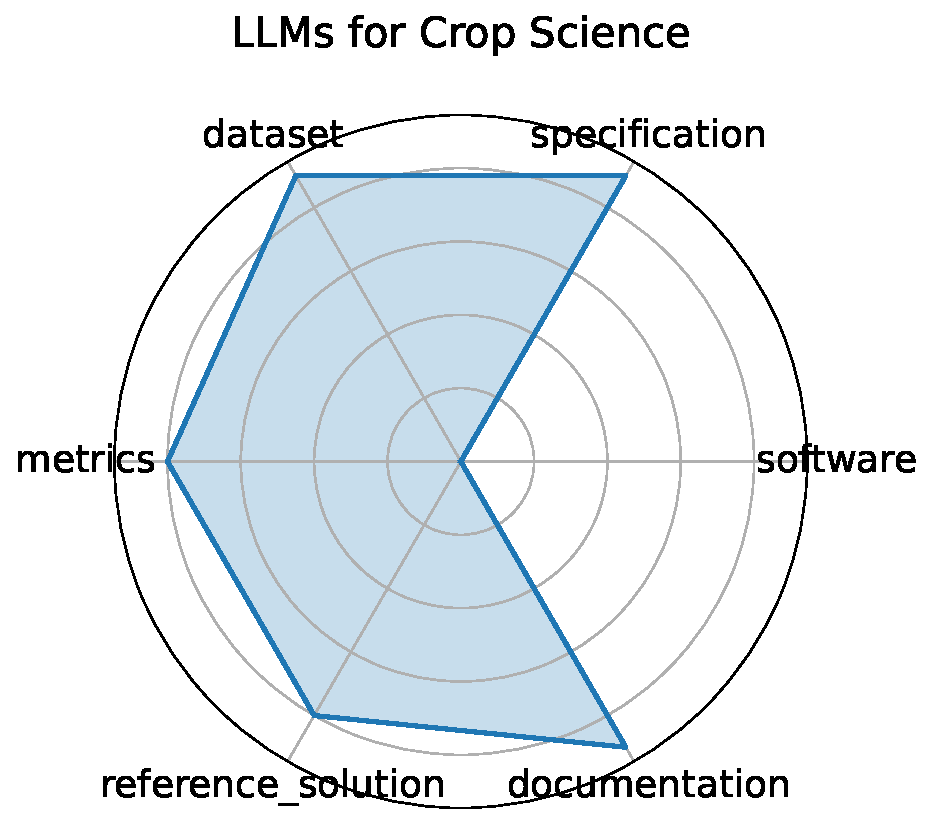
\includegraphics[width=0.2\textwidth]{llms_for_crop_science_radar.pdf}
}}
\clearpage